% This program is free software: you can redistribute it and/or modify
% it under the terms of the GNU AFFERO General Public License as published by
% the Free Software Foundation, either version 3 of the License, or
% (at your option) any later version.
% 
% This program is distributed in the hope that it will be useful,
% but WITHOUT ANY WARRANTY; without even the implied warranty of
% MERCHANTABILITY or FITNESS FOR A PARTICULAR PURPOSE.  See the
% GNU General Public License for more details.
% 
% You should have received a copy of the GNU AFFERO General Public License
% along with this program.  If not, see <https://www.gnu.org/licenses/>.
%
% Copyright (C) 2020 Mo Zhou <cdluminate@gmail.com>
%
\documentclass[9pt,twocolumn,times]{article}
\usepackage{times}
\usepackage[margin=0.9in]{geometry}
\usepackage{tikz}
\usepackage{pgflibraryshapes}
\usetikzlibrary{arrows.meta}
\usepackage{float}
\usepackage{amsmath}
\usepackage{amssymb}
\usepackage{graphicx}
\usepackage{xcolor}
\usepackage{hyperref}
\usepackage{mathtools}
\usepackage{enumitem}
\input{include/math_commands.tex}

\title{Computation Graph Spickzettel}
\author{Mo Zhou\\\small\texttt{<cdluminate@gmail.com>}\\
License: AGPL-3.0}

\begin{document}

\maketitle
\tableofcontents
\newpage

\section{Conventions}

Vectors are column vectors by default.
We follow the naming convention of BLAS/LAPACK for linear algebra operations.
Vecotr, Matrix, Tensor shapes are annotated under the corresponding symbols.
Throughout the whole document, $L$ denotes any loss function (\emph{i.e.},
objective function) of interest.

\section{Automatic Differentiation}

\section{Atomic Modules}

\subsection{Level1: Vector-Vector Ops}

\begin{enumerate}[leftmargin=*]
\item \textbf{Identity} (I)
\begin{equation}
	\underset{(m)}{\vx} = \underset{(m)}{\vy}
\end{equation}
\begin{center}
	\resizebox{0.618\columnwidth}{!}{%
		% This program is free software: you can redistribute it and/or modify
% it under the terms of the GNU AFFERO General Public License as published by
% the Free Software Foundation, either version 3 of the License, or
% (at your option) any later version.
%
% This program is distributed in the hope that it will be useful,
% but WITHOUT ANY WARRANTY; without even the implied warranty of
% MERCHANTABILITY or FITNESS FOR A PARTICULAR PURPOSE.  See the
% GNU General Public License for more details.
%
% You should have received a copy of the GNU AFFERO General Public License
% along with this program.  If not, see <https://www.gnu.org/licenses/>.
%
% Copyright (C) 2020 Mo Zhou <cdluminate@gmail.com>
%
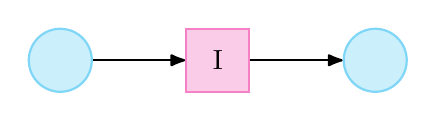
\begin{tikzpicture}[thick,minimum size=8mm]
	\node (x) at (0,0) [circle,draw=cyan!50,fill=cyan!20] {$\vx$};
	\node (ident) at (2,0) [rectangle,draw=magenta!50,fill=magenta!20] {I};
	\node (y) at (4,0) [circle,draw=cyan!50,fill=cyan!20] {$\vy$};
	\draw [-{Latex[round]}] (x) -- (ident);
	\draw [-{Latex[round]}] (ident) -- (y);
\end{tikzpicture}

	}
\end{center}
\begin{equation}
	\underset{(m)}{\frac{\partial L}{\partial \vx}} =
	\underset{(m)}{\frac{\partial L}{\partial \vy}}
\end{equation}

\item \textbf{Transpose} (T)
\begin{equation}
	\underset{(1\times m)}{\vx^T} = \underset{(1\times m)}{\vy}
\end{equation}
\begin{center}
	\resizebox{0.618\columnwidth}{!}{%
		\input{tikz/cg-transpose.tex}
	}
\end{center}
\begin{equation}
	\underset{(m)}{\frac{\partial L}{\partial \vx}} =
	\underset{(m)}{\Big(\frac{\partial L}{\partial \vy}\Big)^T}
\end{equation}

\item \textbf{Addition} (Add)
\begin{equation}
	\underset{(m)}{\vx} + \underset{(m)}{\vz} =
	\underset{(m)}{\vy}
\end{equation}
\begin{center}
	\resizebox{0.618\columnwidth}{!}{%
		\input{tikz/cg-add.tex}
	}
\end{center}
\begin{align}
	\mJ &= \underset{(m\times m)}{\mI} \\
	\underset{(m)}{\frac{\partial L}{\partial \vx}} &=
	\underset{(m)}{\frac{\partial L}{\partial \vy}} \\
	\underset{(m)}{\frac{\partial L}{\partial \vz}} &=
	\underset{(m)}{\frac{\partial L}{\partial \vy}}
\end{align}

\item \textbf{Element-wise Multiplication} (Mul)

\item \textbf{Dot Product} (Dot)

\item \textbf{Element-wise Inverse} (Inv)

\item \textbf{L-2 Norm} (L-2)

\item \textbf{Rectified Linear Unit} (ReLU)

\item \textbf{Sigmoid} ($\sigma$)
\end{enumerate}

\subsection{Level2: Matrix-Vector Ops}

\begin{enumerate}[leftmargin=*]
\item \textbf{GEneral Matrix-Vector multiplication} (GEMV)
\begin{equation}
	\underset{(m\times k)}{\mW} \cdot \underset{(k)}{\vx} =
	\underset{(m)}{\vy}
\end{equation}
\begin{center}
	\resizebox{0.618\columnwidth}{!}{%
		\input{tikz/cg-mv.tex}
	}
\end{center}
\begin{align}
	\underset{(m\times k)}{\frac{\partial L}{\partial\mW}} &=
	\underset{(m)}{\frac{\partial L}{\partial\vy}} \cdot
	\underset{(1\times k)}{\vx^T}\\
	\underset{(k)}{\frac{\partial L}{\partial\vx}} &=
	\underset{(k\times m)}{\mW^T} \cdot
	\underset{(m)}{\frac{\partial L}{\partial \vy}}
\end{align}

\end{enumerate}

\subsection{Level3: Matrix-Matrix Ops}

\begin{enumerate}[leftmargin=*]
\item \textbf{GEneral Matrix-Matrix multiplication} (GEMM)
\begin{equation}
	\underset{(m\times k)}{\mW} \cdot
	\underset{(k\times n)}{\mX} =
	\underset{(m\times n)}{\mY}
\end{equation}
\begin{center}
	\resizebox{0.618\columnwidth}{!}{%
		% This program is free software: you can redistribute it and/or modify
% it under the terms of the GNU AFFERO General Public License as published by
% the Free Software Foundation, either version 3 of the License, or
% (at your option) any later version.
%
% This program is distributed in the hope that it will be useful,
% but WITHOUT ANY WARRANTY; without even the implied warranty of
% MERCHANTABILITY or FITNESS FOR A PARTICULAR PURPOSE.  See the
% GNU General Public License for more details.
%
% You should have received a copy of the GNU AFFERO General Public License
% along with this program.  If not, see <https://www.gnu.org/licenses/>.
%
% Copyright (C) 2020 Mo Zhou <cdluminate@gmail.com>
%
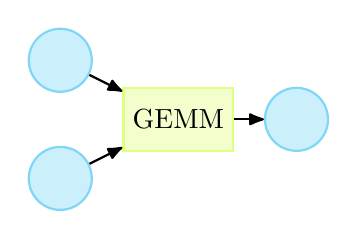
\begin{tikzpicture}[thick,minimum size=8mm]
	\node (w) at (0,0) [circle,draw=cyan!50,fill=cyan!20] {$\mW$};
	\node (x) at (0,-1.5) [circle,draw=cyan!50,fill=cyan!20] {$\mX$};
	\node (gemm) at (1.5,-0.75) [rectangle,draw=lime!50,fill=lime!20] {GEMM};
	\node (y) at (3,-0.75) [circle,draw=cyan!50,fill=cyan!20] {$\mY$};
	\draw [-{Latex[round]}] (w) -- (gemm);
	\draw [-{Latex[round]}] (x) -- (gemm);
	\draw [-{Latex[round]}] (gemm) -- (y);
\end{tikzpicture}

	}
\end{center}
\begin{align}
	\underset{(m\times k)}{\frac{\partial L}{\partial\mW}} &=
	\underset{(m\times n)}{\frac{\partial L}{\partial\mY}} \cdot
	\underset{(n,k)}{\mX^T}\\
	\underset{(k\times n)}{\frac{\partial L}{\partial\mX}} &=
	\underset{(k\times m)}{\mW^T} \cdot
	\underset{(m\times n)}{\frac{\partial L}{\partial \mY}}
\end{align}

\item \textbf{2-D Convolution} (Conv2d)
\end{enumerate}

\section{Network Layers}

\begin{enumerate}[leftmargin=*]
\item \textbf{Affine Transformation Layer} (Affine)

\item \textbf{Mean Square Error} (MSE)
\begin{equation}
	\frac{1}{H} \sum_{i=1}^H
	\|\underset{(n)}{\vx_i} - \underset{(n)}{\hat{\vx}_i} \|_2^2
	= \underset{(1)}{L} 
\end{equation}
\begin{figure}[h]
	\centering
	\resizebox{0.618\columnwidth}{!}{%
		\input{tikz/cg-mse.tex}
	}
	\caption{MSE: $\frac{1}{H} \sum_{i=1}^H \|\vx_i - \hat{\vx}_i\|_2^2 = L$.}
\end{figure}

\item \textbf{Softmax Layer} (Softmax)

\item \textbf{Batch Normalization} (BN)
\end{enumerate}

\section{Networks}

\subsection{Convolutional Neural Networks}

\subsection{Recurrent Neural Networks}

\end{document}
